\documentclass[../../thesis.tex]{subfiles}
\graphicspath{{\subfix{diagrams/}}}

\begin{document}
When launched in 2015, Ethereum \cite{wood2014ethereum} was envisioned as a trustless, permissionless, and decentralized world computer, accessible to anyone. What sets Ethereum apart from other blockchains like Bitcoin \cite{nakamoto2009bitcoin} is the concept of smart-contracts. Smart-contracts are custom, Turing complete programs that are deployed and executed on the Ethereum blockchain in a trustless and permissionless manner. Anybody can interact with these programs by sending transactions to the smart-contract, which results in execution. Smart-contracts can also interact with each other, enabling permissionless composability between them. The technical limitations of this technology have become apparent as well. Computations are expensive, theoretical transactions per second are low, and the overall transaction throughput has been stagnant. While sharding approaches give a direction to scale the network, they are expected to take years to complete. 

\paragraph{Tokenization}
The first major use case for Ethereum was tokenization. With the development of the ERC-20 standard \cite{erc20}, launching a token on the Ethereum blockchain is trivial. As tokens run as smart-contracts on the Ethereum blockchain, they are secured by its proof of work consensus. Given Ethereum's proof of work hash rate, consensus attacks are infeasible. Running on Ethereum blockchain is a significant benefit, as network security can be assumed. Tokenization, however, is also a rather unexciting use case. Most tokens are isolated in their functionality and ecosystem and lack productive usage. 

\paragraph{Decentralized Finance}
A new use case of Ethereum has become apparent in the last months, namely decentralized finance (DeFi). At its core, DeFi protocols aim to productively utilize tokenized assets, somewhat mirroring the traditional financial system in a decentralized fashion. Aave \cite{kulechov_2020} enables lending and collateralized borrowing of tokenized assets. Assets can also be deposited into liquidity pools on Uniswap \cite{adams2020uniswap}, generating yield for the user and enabling decentralized and non-custodial trading. Novel concepts like flash loans have been developed that enable uncollateralized and interest-free loans for the duration of one transaction. It can be questioned how useful or necessary these protocols are. The idea behind them is impressive non the less. As a result of their popularity, these protocols are overwhelming the Ethereum blockchain, increasing the costs of transactions significantly. 

One of these new DeFi applications is Uniswap \cite{adams2020uniswap}. Uniswap is a crypto-asset exchange running as a collection of smart-contracts on the Ethereum blockchain, enabling non-custodial, trustless, and permissionless trading of ERC-20 assets. Uniswap has grown in popularity in recent months, regularly processing over \$1 billion in daily trading volume. The popularity has its toll on the Ethereum blockchain, using around 15\% of Ethereum block space throughout the last months. With the gas price having reached 500 gwei on a couple of occasions, a single Uniswap trade can cost upwards of \$130. While it would be assumed that high gas prices cause a reduction in trading volume, the opposite is the case. As shown in F.\ref{fig:gas_vol} there seems to be a strong correlation between daily trading volume on Uniswap and the average daily Ethereum gas price, so reducing gas consumption by Uniswap transactions should result in a reduced gas price for the entire network.

\begin{figure}[h]
    \centerline{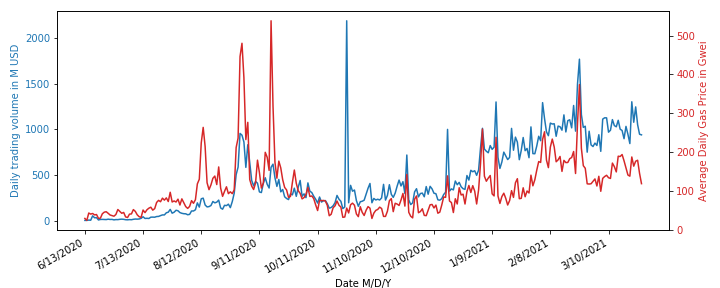
\includegraphics[totalheight=5.6cm]{diagrams/gas_volume.png}}
    \caption{Combined daily Uniswap trading volume average daily Ethereum gas price}
    \label{fig:gas_vol}
\end{figure}


With longer-term scaling solutions in development but still years away, a shorter-term solution is needed. In this work, we will explore zk-rollup as a potential scaling solution for Uniswap trade transactions. The goal is to collect Uniswap trade orders in batches, offset them with each other, and then execute them as one on-chain Uniswap trade. This system aims to remain trustless and permissionless while reducing the transaction cost per trade. Several zk-rollup based applications are running in production, however, in their current state, they are isolated applications that do not rely on other smart-contract interactions to functions. In this work, we will attempt to integrate Uniswap into a custom-built zk-rollup application. The potential issues that arise from being dependant on another application indicate the problems of this approach in general. 


\end{document}